% Chapter 01 - Introduction

\chapter{Introduction}
\label{ch_intro}

\lhead{Chapter \ref{ch_intro}. \emph{Introduction}} % This is for the header on each page - perhaps a shortened title

\clearpage
%----------------------------------------------------------------------------------------

\section{Pancreatic Neoplasia}

\subsection{Epidemiology of pancreatic cancer}
\parencite{crozier_preoperative_2007}
Tumours involving the head of the pancreas and the periampullary region account for a small proportion of gastrointestinal tumours. They may be broadly classified as benign and malignant. Most pancreatic neoplasia are malignant and arise from the exocrine component of the gland, the ductal epithelium. 

Pancreatic ductal adenocarcinoma is the most common cancer of the pancreas. However, the head of the pancreas is anatomically related to several other epithelium lined structures that can also give rise to cancers. These include the distal common bile duct that can give rise to cholangiocarcinoma, the duodenum that can give rise to duodenal adenocarcinoma and the ampulla that can give rise to ampullary adenocarcinoma. The endocrine portion of the pancreas can give rise to a variety of tumours that are collectively called neuroendocrine tumours (NET). The milieu of tumours is complicated by other neoplasia such as intra-ductal papillary neoplasms (IPMN) as well as rare stromal tumours. Occasionally, chronic pancreatitis may present with features similar to pancreatic cancer and can be morphologically, radiologically and histologically difficult to differentiate from cancer.

Pancreatic cancer is the tenth most common cancer in the UK but the fifth most common cause of cancer death with only 21\% surviving beyond the first year and 3\% surviving beyond 5 years.\parencite{cancerresearchuk_cancer_2014} The majority of patients (80-85\%) with pancreatic cancer present with inoperable disease.\parencite{cancerresearchuk_cancer_2014,sener_pancreatic_1999}

In patients with resectable disease, surgery \parencite{sener_pancreatic_1999, sohn_resected_2000,geer_prognostic_1993} followed by adjuvant chemotherapy \parencite{neoptolemos_randomized_2004, neoptolemos_adjuvant_2009} remains the primary modality of cure. However, major pancreatic surgery places significant physiological stresses on multiple organ systems. The ability of the cardiac and respiratory systems, in particular, to cope with the increased physiological demand placed by general anaesthesia and major pancreatic surgery plays an important role in determining outcome after surgery.

\subsection{Clinical presentation}

The anatomical location of the pancreas, deep within the retroperitoneum surrounded by numerous vital blood vessels including the coeliac trunk and its branches, the superior mesenteric artery, portal vein and superior mesenteric vein as well as proximity to other viscera such as the stomach, duodenum, transverse colon result in early involvement of these structures even by relatively small tumours. Moreover, symptoms are often absent in the early stages and when present are too non-specific to help with diagnosis. Obstructive jaundice is the most common presenting symptom and painless, obstructive jaundice in an elderly patient should always raise the suspicion of a neoplastic process in the head of the pancreas or the periampullary region. Other non-specific symptoms include weight loss, early satiety, vomiting, fatigue and pain in the epigastrium or the back. 
 
\subsection{Diagnosis and staging}

Aside from a thorough history, clinical examination, blood tests including liver function tests, diagnosis requires cross-sectional imaging in the form of a contrast-enhanced computerised tomogram (CECT) of the abdomen using a pancreas-specific protocol (a modified form of the portal-venous phase). CECT of the pancreas when combined with CT Thorax also provides accurate information on staging of the disease with regards to metastasis and this can be supplemented by further imaging such as Positron Emission Tomography (PET-CT) or contrast-enhanced MRI Liver in specific cases. CECT-pancreas is also useful for assessing local resectability with regards to vascular involvement. Endoscopic ultrasound (EUS) is also useful in assessing vascular involvement and for obtaining tissue samples for histological examination. In jaundiced patients, endoscopic retrograde cholangio pancreatography (ERCP) plays an important role in the alleviation of jaundice by placing stents across the obstructed bile ducts, accurate visualisation of the biliary anatomy as well as obtaining brushings from within the bile ducts for cytological examination. The role of preoperative biliary drainage is discussed in more detail in section %\ref{sec:preoperative_biliary_drainage].
	
\subsection{Treatment of pancreatic cancer}
Pancreaticoduodenectomy followed by adjuvant chemotherapy offers the only chance of cure in patients with resectable pancreatic cancer who are fit enough to undergo surgery. In patients with unresectable disease or who are not fit to undergo surgery, palliative chemotherapy plays a limited role in prolonging survival. Assessing the resectability is discussed in the next section while the assessment of patient fitness and the impact of comorbidity are discussed in detail in section \ref{sec:comorbidity_risk_stratification} on p\pageref{sec:comorbidity_risk_stratification}.

\section{Surgical treatment of pancreatic cancer}
Pancreaticoduodenectomy remains a technically challenging and complex surgical procedure over a hundred years after its description. The procedure was performed as a two-stage operation by a German surgeon, Walther Kausch in 1909 at Augusta-Viktoria-Krankenhaus in Berlin-Schöneberg.\parencite{kausch_carcinom_1912}. The operation was further popularised initially as a two-stage procedure by Whipple\parencite{whipple_treatment_1935} before evolving into the current single stage operation by the 1950s.\parencite{whipple_rationale_1941,whipple_radical_1950}

\subsection{Patient selection}
\subsubsection{Resectability criteria}
Resectable pancreatic cancer is defined as a tumour that
- does not involve the coeliac axis or the superior mesenteric artery
- and is not associated with distant metastatic disease

Tumours involving the portal vein or superior mesenteric vein are considered borderline resectable and can still be resected completely (R0) with en-bloc venous resection. Research is ongoing to assess the role of neoadjuvant therapy and newer treatment modalities such as electroporation in these patients to improve resectability.

\subsubsection{Patient factors}
\subsection{Operative technique}
Pancreaticoduodenectomy is considered one of the most technically challenging operations on the gastrointestinal tract. While the procedure is carried out in a broadly similar fashion in all major centres, there remain some variations in perioperative care as well as some operative steps. The following is a description of the procedure as performed at the West of Scotland Pancreatic Unit.

After a comprehensive preoperative work-up including both assessments of the tumour as well as patient fitness, informed consent was obtained. Patients received thrombo-prophylaxis on the night before surgery which was continued until discharge from hospital. General anaesthesia with complete muscle relaxation was used in all patients. Epidural analgesia was used routinely in patients during the early part of the study period while all patients in the later half of the study period received spinal diamorphine. Antibiotic prophylaxis is administered at induction. While the use of Octreotide, a somatostatin analogue, to reduce the risk of postoperative pancreatic fistula formation is still debated, it was routinely used in all patients at this centre. Octreotide was administered intra-operatively (200 mcg s.c.) and was continued for 5 days postoperatively (200 mcg s.c., t.d.s.).

A roof-top incision was used for access. After assessing the peritoneal cavity for absence of metastatic disease, an early assessment was made for local resectability. This involved complete Kocherisation of the duodenum to assess the retroperitoneum. Both the superior mesenteric artery and coeliac axis were assessed early for tumour involvement (‘artery-first’ approach). The rest of the procedure was performed as described extensively elsewhere. The gastrocolic omentum was divided to enter the lesser sac. The superior mesenteric vein was identified and a retro-pancreatic tunnel was created between the pancreatic neck and the portal vein. If less than half the circumference of the SMV or PV was involved, an en-bloc resection was performed with vein repair at the same time. The hepatoduodenal ligament was dissected after a fundus-first cholecystectomy to isolate the common bile duct which was transected after ascertaining the hepatic artery anatomy. The gastro-duodenal artery was divided. Resection was then completed by dividing the stomach (classical Whipple procedure) or the first part of the duodenum (pylorus-preserving pancreaticoduodenectomy, PPPD) and transecting the pancreatic neck.

Reconstruction was performed as follows: Either a pancreatico-jejunostomy was performed using 4-0 Biosyn sutures in a two-layer duct-to-mucosa technique or a pancreatico-gastrostomy was performed using 3/0 Biosyn sutures placed in a similar manner. Hepaticojejunostomy was performed using interrupted 4/0 Biosyn sutures while the gastrojeunonostomy or duodenojejunostomy (in PPPD) was performed using continuous 3/0 PDS sutures in a 2-layers. One or two surgical drains were placed and the abdomen was closed after ensuring haemostasis.

\subsection{Postoperative care}
All patients were routinely admitted to the Surgical High Dependency Unit unless intra-operative events necessitated admission to the Intensive Care Unit. A standardised regimen of intravenous fluids, naso-jejunal feeding, mobilisation and physiotherapy was implemented in all patients. Standard physiological parameters including haemodynamic parameters, renal function and arterial blood gases were used to monitor adequate end organ perfusion. All patients received proton pump inhibitors and octreotide. Patients were discharged to the general surgical ward as early as possible.

\subsection{Complications}
The incidence of complications after pancreaticoduodenectomy remains high in spite of a steady decline in postoperative mortality from over 40\% in the 1950's to less than 5\% in most large volume centres around the world.\parencite{deoliveira_assessment_2006,emick_hospital_2006,yeo_six_1997, winter_1423_2006,teh_patient_2009,gouma_rates_2000}

\subsubsection{Postoperative pancreatic fistula}
Postoperative pancreatic fistula is one of the most dreaded complications after a pancreaticoduodenectomy and can be associated with significant short-term morbidity as well as long-term disability. The reported incidence of postoperative pancreatic fistula varies from 2\% to 30\% after pancreaticoduodenectomy.\parencite{yeo_six_1997,deoliveira_assessment_2006,bassi_postoperative_2005,winter_biochemical_2007,pratt_risk_2008} 
The variation in reported incidence has been largely due to lack of clear definition of what constituted a postoperative pancreatic fistula. It can be a result of breakdown or poor healing at the pancreaticojejunostomy/pancreaticogastrostomy or may be the result of direct parenchymal leak unrelated to the anastomosis. It is now generally accepted that 1 in 4 patients will develop a pancreatic fistula as defined by the International Study Group for Pancreatic Fistula (ISGPF) which has published a consensus statement on the definition and grading of postoperative pancreatic fistula.\parencite{bassi_postoperative_2005} A postoperative pancreatic fistula is defined as drain output of any measurable quantity after the third postoperative day with amylase content greater than three times the upper limit of the normal serum amylase value at the laboratory used for testing. Three grades of postoperative pancreatic fistula have been defined based on clinical severity as described in Table \ref{table:isgps_popf} on p\pageref{table:isgps_popf}. Grade B and C fistulae are considered to be clinically significant in that they alter patient management and are often associated with other secondary complications such as intra-abdominal sepsis, post-pancreatectomy haemorrhage, delayed gastric emptying as well as need for intervention (either radiological or operative) and/or prolonged critical care support.

\subsubsection{Post-pancreatectomy haemorrhage}
Post-pancreatectomy haemorrhage is reported to occur in 1 to 8\% of patients undergoing pancreaticoduodenectomy. However, it accounts for 11\% to 38\% of mortality after pancreaticoduodenectomy. Post-pancreatectomy haemorrhage may either be intra-luminal into the gastrointestinal tract or intra-abdominal into the peritoneal/retro-peritoneal space. Post-pancreatectomy haemorrhage may be from any of a number of potential sources although bleeding from the stump of the gastroduodenal artery is the most common cause. Other potential sources include suture lines at the anastomoses, gastric/duodenal ulcers or diffuse gastritis, pseudoaneurysms of the gastro-duodenal, splenic or rarely the hepatic artery or rarely, haemobilia.

Haemorrhage is often secondary to non-healing of the pancreatico-jejunal anastomosis leading to leakage of amylase-rich pancreatic juices into the retroperitoneum or secondary to intra-abdominal sepsis or bile leak.\parencite{tien_risk_2005, koukoutsis_haemorrhage_2006, choi_delayed_2004, balladur_bleeding_1996} This can then lead to erosion of ligated blood vessels, most commonly the stump of the gastro-duodnenal artery. Post-pancreatectomy haemorrhage is often managed with angiographic embolisation of the bleeding vessel and surgical intervention is only rarely required. The grading of severity of post-pancreatectomy haemorrhage as described by the International Study Group of Pancreatic Surgery\parencite{wente_postpancreatectomy_2007} is shown in Table \ref{table:isgps_pph} on p\pageref{table:isgps_pph}.

\begin{sidewaystable}[htbp]
\centering
\caption{Postoperative pancreatic fistula: ISGPF definition.}
\label{table:isgps_popf}
\begin{tabular}{|m{4cm}|m{4cm}|m{5cm}|m{5cm}|}
	\hline
	Grade                                & A        & B                 & C                 \\ \hline
	Clinical conditions                  & Well     & Often well        & Ill appearing/bad \\
	Specific treatment                   & No       & Yes/no            & Yes               \\
	US/CT (if obtained)                  & Negative & Negative/positive & Positive          \\
	Persistent drainage (after 3 weeks)† & No       & Usually yes       & Yes               \\
	Reoperation                          & No       & No                & Yes               \\
	Death related to POPF                & No       & No                & Possibly yes      \\
	Signs of infections                  & No       & Yes               & Yes               \\
	Sepsis                               & No       & No                & Yes               \\
	Readmission                          & No       & Yes/no            & Yes/no            \\ \hline
\end{tabular}

\caption{Postpancreatectomy haemorrhage: ISGPS definition.}
\label{table:isgps_pph}
\begin{tabular}{|m{4cm}|m{4cm}|m{5cm}|m{5cm}|}
	\hline
	Grade                                                             & A                                                                                & B                                                                                                                             & C                                                                                         \\ \hline
	Time of onset, location, severity and clinical impact of bleeding & Early, intra- or extraluminal, mild                                              & Early, intra- or extraluminal, severe	or Late, intra- or extraluminal, mild                                                   & Late, intra- or extraluminal, severe                                                      \\
	Clinical condition                                                & Well                                                                             & Often well/ intermediate, very rarely life-threatening                                                                        & Severely impaired, life-threatening                                                       \\
	Diagnostic consequence                                            & Observation, blood count, ultrasonography and, if necessary, computed tomography & Observation, blood count, ultrasonography, computed tomography, angiography, endoscopy                                        & Angiography, computed tomography, endoscopy                                               \\
	Therapeutic consequence                                           & No                                                                               & Transfusion of fluid/blood, intermediate care unit (or ICU), therapeutic endoscopy,† embolization, relaparotomy for early PPH & Localization of bleeding, angiography and embolization, (endoscopy†) or relaparotomy, ICU \\ \hline
\end{tabular}
\end{sidewaystable}

\subsubsection{Clavien-Dindo classification of complications}
A number of other adverse events may occur following pancreaticoduodenectomy including cardiopulmonary complications such as myocardial infarction, cardiac arrythmias, pneumonia, pleural effusions, wound complications such as wound sepsis and dehiscence, intra-abdominal sepsis including intra-abdominal sepsis, leakage from the hepaticojejunostomy or the gastrojejunostomy, renal dysfunction, etc. The Clavien-Dindo method grades the severity of complications based on the impact the complication has on the management of the patient and has been validated on large numbers of surgical patients.\parencite{clavien_clavien-dindo_2009, dindo_classification_2004} This is summarised in Table \ref{table:clavien-dindo} on p\pageref{table:clavien-dindo} and has been used to grade complications in this thesis.

\begin{sidewaystable}[htbp]
	\centering
	\caption{The Clavien-Dindo classification of surgical complications.}
	\label{table:clavien-dindo}	
	\renewcommand{\arraystretch}{1.7} %Increases space between rows
	\setlength{\tabcolsep}{14pt} %sets the space between columns
	\begin{tabular}{|l m{15cm}|}
		\hline
		Grade       & Description \\ \hline
		Grade I     & Any deviation from the normal postoperative course without the need for pharmacological treatment or surgical, endoscopic and radiological interventions.  \\
		Grade II    & Requiring pharmacological treatment with drugs other than such allowed for grade I complications. Blood transfusions and total parenteral nutrition are also included.  \\
		Grade III   & Requiring surgical, endoscopic or radiological intervention  \\
		            & Grade III-a: - intervention not under general anaesthesia \\
		            & Grade III-b: - intervention under general anaesthesia  \\
		Grade IV    & Life-threatening complication (including CNS complications)‡ requiring  HDU/ICU-management  \\
		            & Grade IV-a: - single organ dysfunction (including dialysis)     \\
		            & Grade IV-b: - multi organ dysfunction \\
		Grade V     & Death of a patient  \\ \hline
		Suffix 'd': & If the patient suffers from a complication at the time of discharge,  the suffix  “d”  (for ‘disability’) is added to the respective grade of complication. This label indicates the need for a follow-up to fully evaluate the complication. \\ \hline
	\end{tabular}
\end{sidewaystable}



 	


\section{Adjuvant and Neoadjuvant treatment}

\clearpage

\section{Comorbidity and Risk Stratification}
\label{sec:comorbidity_risk_stratification}
\subsection{Comorbidity}
Comorbidity is defined as the presence of or the effect of other diseases that a patient has in addition to the primary disease of interest. The presence of comorbid conditions is associated with adverse outcomes in patients undergoing treatment for pancreatic cancer\parencite{mann_review_2010} and often limits therapeutic options available due to the associated complications or side effects of surgery or chemoradiotherapy.\parencite{sandroussi_sociodemographics_2010}

Patients with multiple comorbidities are more likely to have higher readmission rates, morbidity and mortality following discharge after pancreaticoduodenectomy.\parencite{schneider_patient_2012} DeOliveira and co-workers reported that cardiovascular disease was a risk factor not only for overall morbidity but also complication severity after pancreaticoduodenectomy.\parencite{deoliveira_assessment_2006} Cancer cachexia is associated with increased incidence of complications and mortality after pancreaticoduodenectomy\parencite{pausch_cachexia_2012} while obesity is known to be associated with greater incidence and severity of postoperative complications.\parencite{benns_impact_2009}

Major pancreatic surgery requires the patient to have adequate physiological reserve to cope with the increased demand during and immediately after surgery. However, existing methods of measuring the impact of comorbidity on physiological fitness are limited and do not adequately predict outcomes after major pancreatic surgery. \parencite{shah_limitations_2012}

\subsection{Risk Stratification}
Physiological fitness or reserve may be defined as the ability of the patient’s organ systems to respond appropriately and adequately to the stress of major surgery. Major surgery places a significant physiological stress on multiple organ systems, especially the cardiorespiratory system. The ability of the cardiorespiratory system as well as other physiological systems including renal, gastrointestinal, hepatic, coagulatory and immunological systems to cope with major surgery and the postoperative recovery plays a major role in determining short-term outcomes. 

Accurate measurement of physiological fitness 

\subsection{Static Versus Dynamic Testing}

Objective measurement of oxygen delivery at the tissue level at times of physiological stress allows for identification of patients who may struggle during the perioperative phase. Identification of such high-risk patients allows not only for improved patient selection, but also for risk-stratified, anaesthetic and postoperative critical care. Preoperative risk stratification will also allow for prehabilitation of these patients in an attempt to improve outcomes. 

Several tests have been used for preoperative assessment of cardiac function. These include 
- electrocardiography 
- echocardiography 
- exercise tolerance testing 
- myocardial perfusion scans 

Tests of respiratory function that are commonly performed in selected patients undergoing major surgery include 
- pulmonary function tests including forced expiratory volume and forced vital capacity 
- spirometry 

However, neither of the above cardiac or respiratory function tests adequately measure the ability of the cardiopulmonary and circulatory systems to deliver oxygen to the tissues at times of increased demand.

\section{Cardiopulmonary Exercise Testing}
%History of CPET
\subsection{History of CPET in Surgery}

\subsection{Cardiopulmonary Exercise Test Methodology}
CPET is composed of several components that involve measuring not only the response of the cardiac and respiratory system to exercise but the test also helps establish the adequacy of this response to sustain oxygen delivery to skeletal muscle as demand increases with increasing exercise. 

Cardiopulmonary exercise tests were performed in the Department of Respiratory Medicine at the Glasgow Royal Infirmary using the ZAN-600 CPET suite (nSpire Health, Longmont, CO 80501, USA). The equipment was calibrated regularly to the standards set by the manufacturer and currently published guidelines[]. All tests were performed by specialist respiratory physiologists. Suitable equipment for cardiopulmonary resuscitation were available in the department in case of unexpected problems. The department was situated within the main hospital premises and therefore was easily accessible to the hospital cardiac arrest team. All patients were fully informed of the steps involved in the procedure, the reasons for performing the test as well as the risks involved. 

Spirometry was performed in all patients prior to CPET. Capillary blood gases were measured in all patients after CPET. An electronically braked cycle ergometer was used to increase resistance to pedalling in preset increments. A tight-fitting face mask was placed on the patient covering the nose and the mouth. This allowed breath-by-breath gas analysis thus allowing measurement of several respiratory parameters as listed in table []. 12-lead electocardiogram was recorded at the same time. 

The test started with an initial 3-minute rest period to allow measurement of baseline parameters. This was followed by an incremental work-load test that involved the patient pedalling approximately at 60 revoultions per minute while the resistance to pedalling was gradually increased in preset increments. The test was terminated when patients reached volitional fatigue (maximal exercise tolerance), significant ischaemic changes on ECG or for other safety reasons. 

The parameters measured at spirometry are shown in Table \ref{table:spirometry} and those measured during cardiopulmonary exercise testing are shown in Table \ref{table:cpet_parameters} on p\pageref{table:cpet_parameters}.

\subsection{Measuring the Anaerobic Threshold}
The anaerobic threshold (variously described as the lactate threshold or ventilatory threshold) is the point during exercise when oxygen demand by exercising skeletal muscle outstrips supply. Therefore, muscle tissues use anaerobic respiration to supplement aerobic respiration to continue generation of ATP. The resulting metabolic lactic acidosis is almost immediately compensated by the bicarbonate buffer as below: 
\begin{equation} \label{eq:bicarb_buffer}
	H^+ + HCO3^- \Longleftrightarrow H_2CO_3 \Longleftrightarrow H_2O + CO_2
\end{equation}
The resulting excess $CO_2$ is exhaled and is one of the many parameters measured during cardiopulmonary exercise testing. This transition from aerobic to anaerobic respiration may be determined using the V-slope method\parencite{sue_metabolic_1988} or the ventilatory equivalents method.\parencite{beaver_new_1986} Most centres, like ours, use both methods supplemented by information from a variety of other parameters to enable accurate determination of the anaerobic threshold as recommended by the American Thoracic Society/American College of Chest Physicians Statement on cardiopulmonary exercise testing.\parencite{society_ats/accp_2003}

The software presents a standard 9-panel view of trending plots of various parameters measured during incremental exercise. All of these trends are taken into consideration rather than any one particular parameter value in determining the overall outcome of the test. A sample 9-panel view derived from parameters belonging to one of the patients studied is shown in Figure \ref{fig:cpet_9panel}. The data used to generate these plots is included in Appendix \ref{AppendixCPETRawData}. 

\begin{figure}[p]
	\centering
	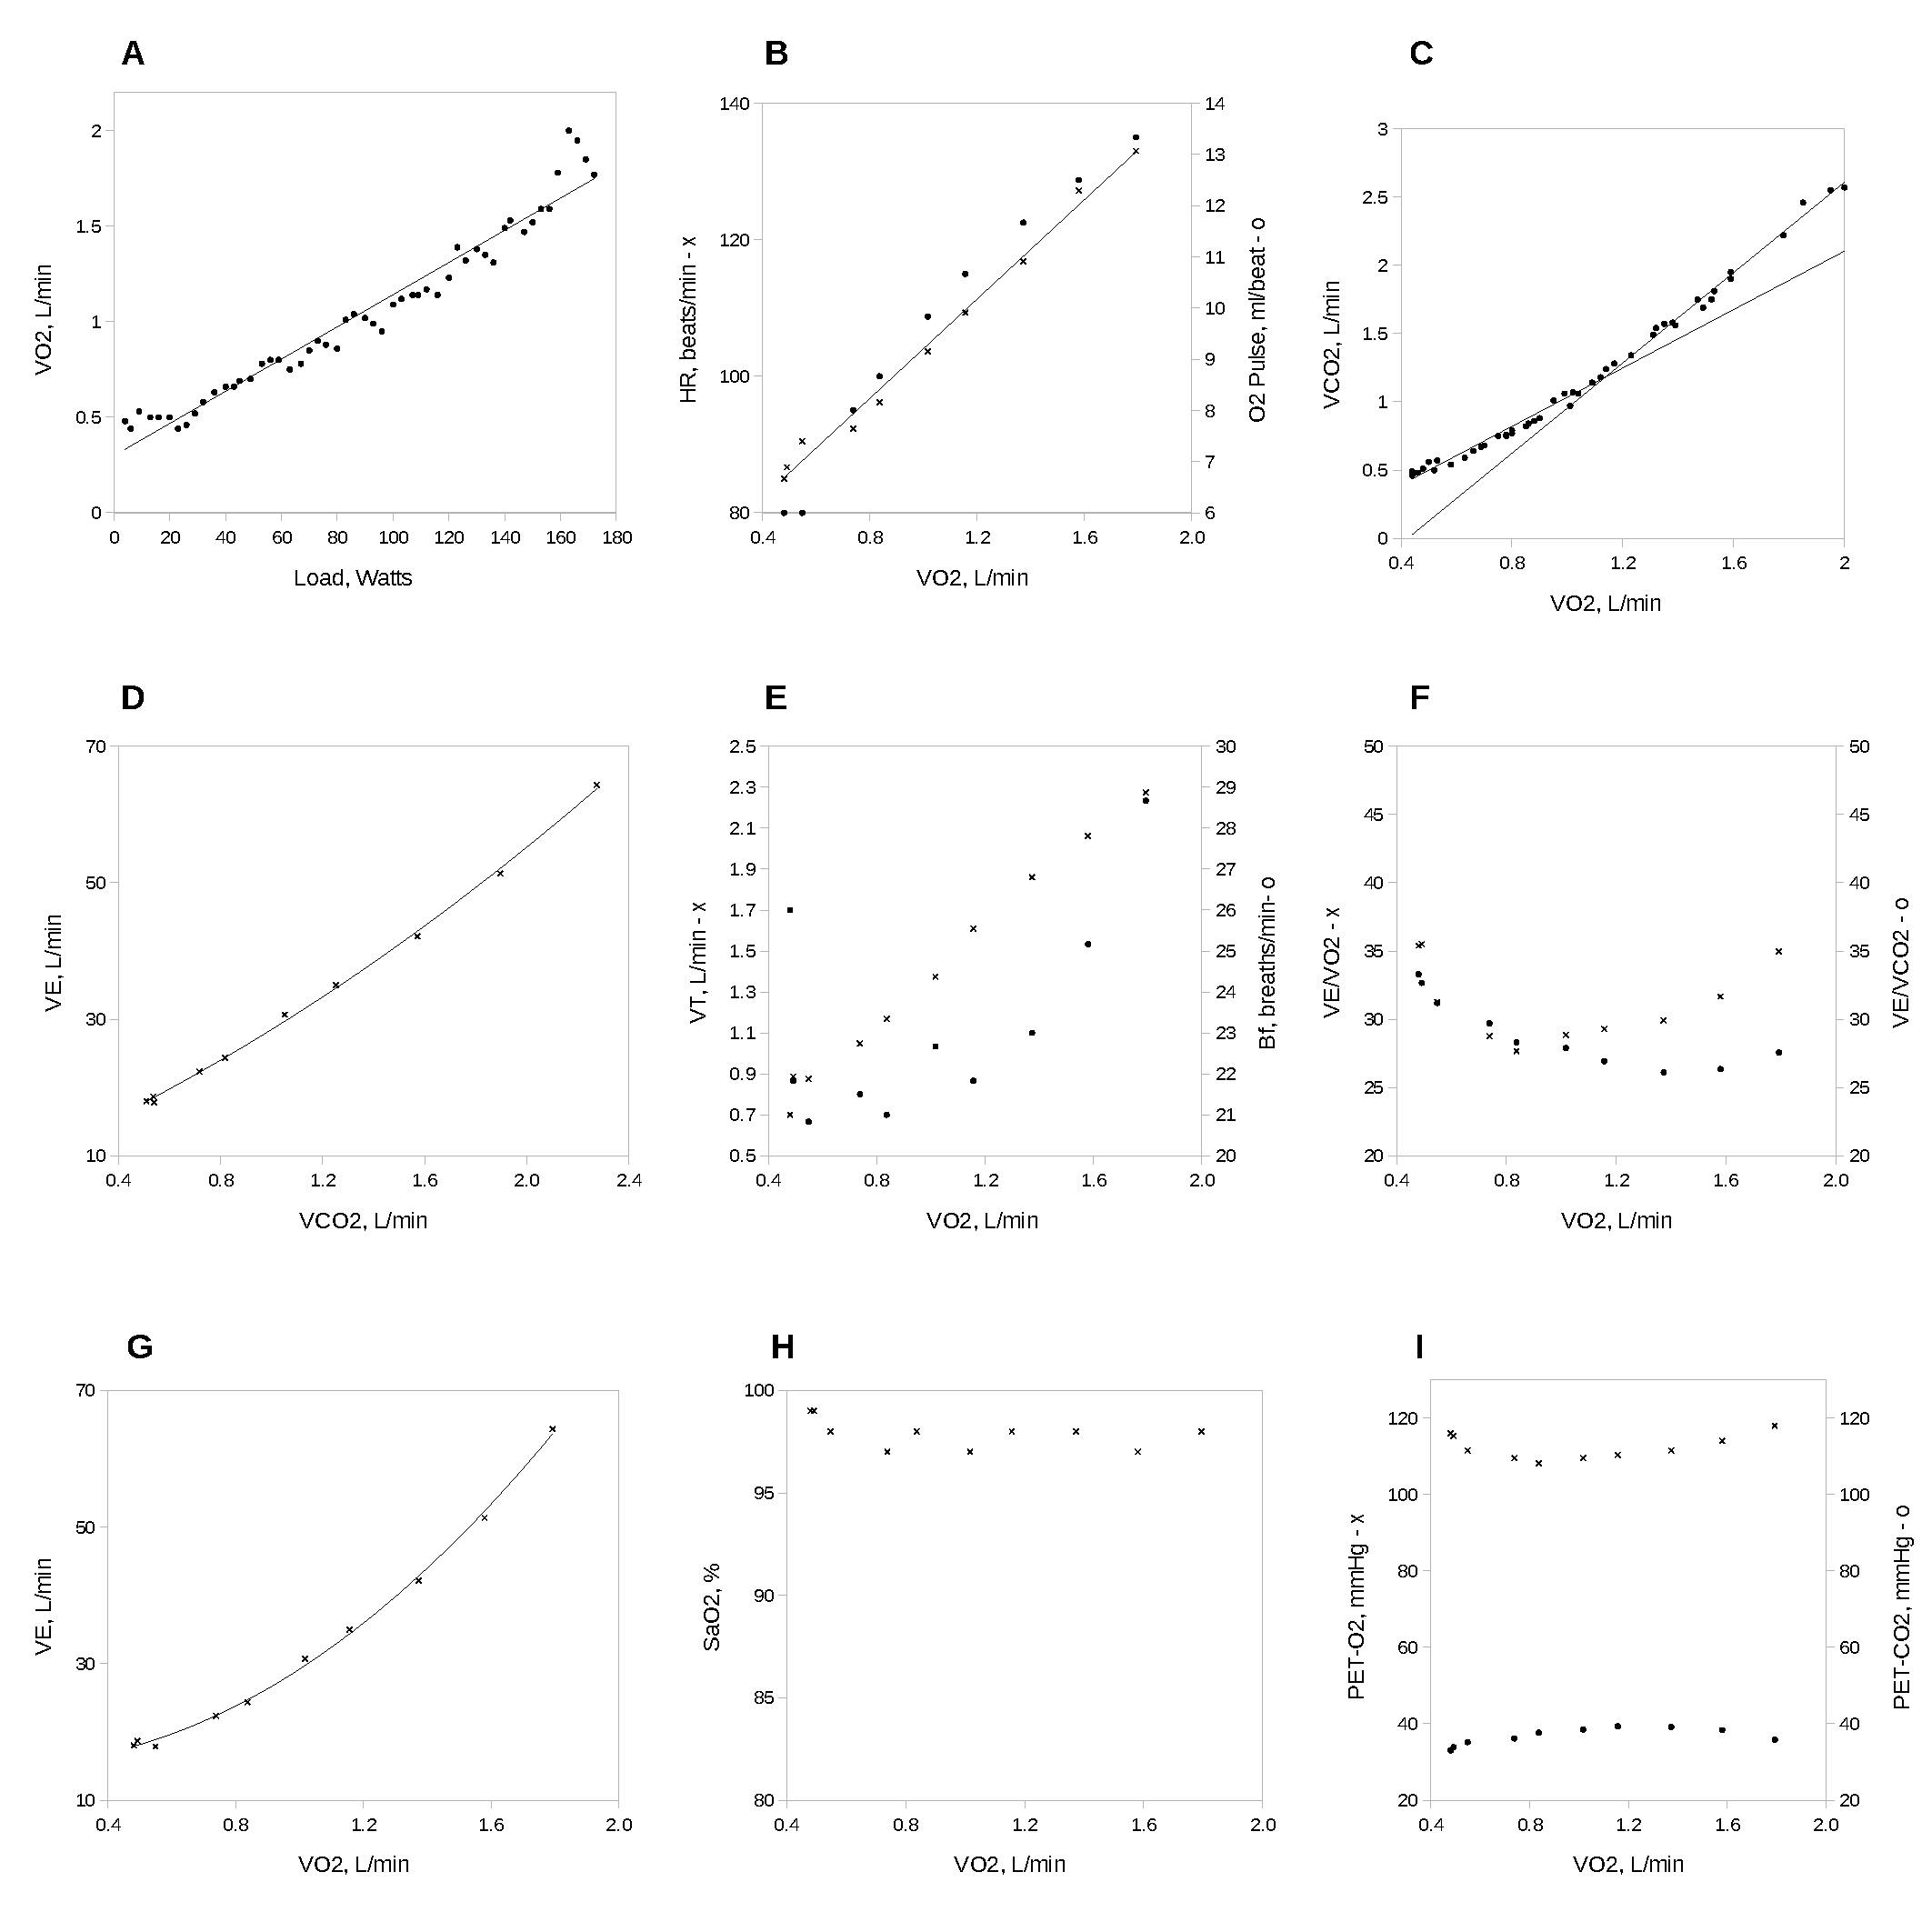
\includegraphics[width=0.9\textwidth]{Figures/cpet_9panel.pdf}
	\caption{9-panel view of trending parameters during incremental cardiopulmonary exercise.}
	\label{fig:cpet_9panel}
\end{figure}


\subsubsection{V-slope method}

During aerobic exercise, VO2 and VCO2 share a linear relationship as shown in segment A of the graph in figure 1. However, as anaerobic respiration starts to supplement aerobic respiration, VCO2 increases disproportionate to VO2 as a direct result of the respiratory buffer described in equation \ref{eq:bicarb_buffer} on p\pageref{eq:bicarb_buffer}. This results in a distinct difference in the slope of the initial part of the graph (seg A) and the later part (seg B). The point at which the two slopes intersect is the anaerobic threshold and the V02 at this point in exercise is commonly referred to as the anaerobic threshold, VO2at or simply AT. 


\subsubsection{Ventilatory equivalents method}
[...] 

\section{Description of CPET Parameters}
\begin{table}[p]
\centering
\caption{Parameters measured at spirometry.}
\label{table:spirometry}
\begin{tabular}{| m{2cm}  m{2cm}  m{7cm} |}
	\hline
	Parameter & Units  & Description                          \\ \hline
	FVC       & litres & Forced Vital Capacity                \\
	FEV1      & litres & Forced Expiratory Volume in 1 second \\
	FEV1/FVC  & \%     & Tiffeneau-Pinelli[1] index           \\ \hline
\end{tabular}

\vspace{2cm}


\caption{Common parameters measured at cardiopulmonary exercise testing.}
\label{table:cpet_parameters}
\begin{tabular}{| m{2cm}  m{2cm}  m{7cm} |}
	\hline
	Parameter & Units       & Description                                  \\ \hline
	\%peakVO2 & \%          & VO2 as a \% of predicted VO2Peak             \\
	Load      & Watts       & Exercise Workload                            \\
	VE        & litres/min  & Ventilatory Equivalent                       \\
	Vt        & litres      & Tidal volume                                 \\
	VO2       & litres/min  & Absolute Oxygen uptake/consumption           \\
	VO2/kg    & ml/(kg*min) & Corrected Oxygen uptake/consumption          \\
	VE/VO2    &             & Ventilatory Equivalent for O$_2$             \\
	VCO2      & litres/min  & Carbon-dioxide output                        \\
	VE/VCO2   &             & Ventilatory Equivalent for CO$_2$            \\
	RER       &             & Respiratory Exchange Ratio                   \\
	PETO2     & mmHg        & End Tidal O2                                 \\
	PETCO2    & mmHg        & End Tidal CO2                                \\
	O2Pulse   & ml/beat     & Oxygen pulse                                 \\
	HR        & beats/min   & Heart Rate                                   \\
	Bf        & /min        & Breathing Frequency                          \\
	P(A-a)O2  & mmHg        & Alveolar-arterial PO2 difference             \\
	Vd/Vt     &             & Physiologic dead space-to-tidal volume ratio \\
	SBP       & mmHg        & Systolic blood pressure                      \\
	DBP       & mmHg        & Diastolic blood pressure                     \\
	O2sat     & \%          & Oxygen saturation                            \\ \hline
\end{tabular}

\end{table}


\subsection{Exercise Load}
The most common form of cardiopulmonary exercise testing for clinical purposes involves a cycle ergometer with steadily increasing resistance delivered through electric braking allowing accurate measurement of work load in Watts. The relationship between $\dot{V}_{O_2}$ and work rate is usually linear and the slope of this relationship is independent of sex, age or height. An abnormality in this relationship is usually due to cardiopulmonary or circulatory causes.

\subsection{Minute Ventilation, $\dot{V}_E$}
Minute ventilation or respiratory minute volume is the volume of air that is inhaled/expired in a minute.
\begin{equation} \label{eq:VE=VTxBf}
	\dot{V}_E = \dot{V}_T \times Bf
\end{equation}
where $\dot{V}_T$ = Tidal Volume and $Bf$ = Breathing Frequency.

Increasing $\dot{V}_E$ is one of the main mechanisms involved in increasing oxygen delivery during exercise. It is also an important factor in clearing $CO_2$ from the blood.

\subsection{Oxygen Uptake, $\dot{V}_{O_2}$}

$\dot{V}_{O_2}$ or oxygen uptake is measured breath-by-breath using digital analysis of the inspired and expired gases. This is then averaged, usually over time, to smooth-out any signficant breath-by-breath variation. $\dot{V}_{O_2}$ increases with increasing work load and is influenced by several factors that have a role in the transport and utilisation of oxygen. These may be broadly classified as cardiac, pulmonary, circulatory and tissue factors. Some of the factors are encompassed in the following formula for $\dot{V}_{O_2}$.
\begin{equation} \label{eq:VO2=CaO2xCO}
	\dot{V}_{O_2} = CaO_2 \times Cardiac\ Output
\end{equation}
where $CaO_2$ is $O_2$ content per ml of blood and is defined by,
\begin{equation} \label{eq:CaO2=Hbx1.34xSaO2}
	CaO_2 = Haemoglobin \times 1.34 \times SaO_2
\end{equation}
and
cardiac output, the primary cardiac factor that influences $\dot{V}_{O_2}$, is:
\begin{equation} \label{eq:CO=SVxHR}
	Cardiac\ Output = Stroke\ Volume \times Heart\ Rate
\end{equation}
Stroke volume is in turn influenced by ventricular function and end-diastolic volumes. The heart rate response to exercise is discussed in section \ref{sec:heart_rate} on p\pageref{sec:heart_rate}.

Pulmonary gas exchange plays an important role in the oxygenation of blood and removal of $CO_2$ and is influenced by numerous factors, the detailed discussion of which is beyond the scope of this chapter. However, ventilation, pulmonary blood flow, gas-exchange across the alveolar membrane and ventilation-perfusion mismatches (V/Q mismatch) all play an important role in determining the response of the lungs to exercise.

The quality of the peripheral circulation, both anatomical and its physiologic response to exercise which involves redistribution of blood flow to exercising muscle, has an important role in increasing availability of oxygen. The oxygen carrying capacity of blood determined by haemoglobin concentration, its saturation and the $O_2$ dissociation curve as well as the ability of tissues to extract and utilise oxygen are equally important factors that influence $\dot{V}_{O_2}$.

\subsection{Oxygen Pulse, $O_2Pulse$}
Oxygen pulse is defined as the oxygen uptake per heart beat.
\begin{equation} \label{eq:O2Pulse=VO2/HR}
	O_2Pulse = \frac{\dot{V}_{O_2}}{Heart\ rate}
\end{equation}
While some authors have suggested that oxygen pulse may be a surrogate for stroke volume others disagree. The clinical application of oxygen pulse in surgical patients remains unclear.

\subsection{Respiratory Exchange Ratio, RER}
The ratio of $\dot{V}_{CO_2}/\dot{V}_{O_2}$ is called the Respiratory Exchange Ratio. An RER greater that 1.0 may be caused either by lactic acidosis or due to hyperventilation. The RER is also a marker of the fuel being used for metabolism with RER less than 1.0 indicating mixed fuel source in the form of carbohydrate and fat while an RER of 1.0 or greater indicates a primarily carbohydrate source.

\subsection{Ventilatory Equivalent for $O_2$ and $CO_2$, $\dot{V}_E/\dot{V}_{O_2}$, $\dot{V}_E/\dot{V}_{CO_2}$}
The change in $\dot{V}_E/\dot{V}_{O_2}$ and $\dot{V}_E/\dot{V}_{CO_2}$ during exercise provide valuable information regarding the ventilatory response to exercise. Both $\dot{V}_E/\dot{V}_{O_2}$ and $\dot{V}_E/\dot{V}_{CO_2}$ tend to decrease initially during exercise. However, as the anaerobic threshold is passed, $\dot{V}_E/\dot{V}_{O_2}$ starts increasing before $\dot{V}_E/\dot{V}_{CO_2}$. This change in direction is yet another method to confirm the anaerobic threshold.  $\dot{V}_E/\dot{V}_{CO_2}$ eventually starts increasing as well as respiratory compensation of metabolic acidosis results in increased $\dot{V}_E$.

\subsection{End-tidal $O_2$ and $CO_2$, $P_{ET_{O_2}}$, $P{ET_{CO_2}}$}
$PET_{O_2}$ and $PET_{CO_2}$ are the partial pressures of $O_2$ and $CO_2$ at the end of an exhaled breath and are closely related to PaO2 and PaCO2 respectively. $P{ET_{CO_2}}$ is dependent on pulmonary gas-exchange which is in turn influenced by the right ventricular output, pulmonary blood flow and alveolar gas exchange. The changes in $P_{ET_{O_2}}$ and $P{ET_{CO_2}}$ during exercise help identify ventilation-perfusion mismatch as well as hyperventilation.

\subsection{Heart Rate, HR}
\label{sec:heart_rate}
The heart rate response during exercise in healthy individuals is a linear function of $\dot{V}_{O_2}$ increasing linearly with increasing work load and increasing $\dot{V}_{O_2}$. The difference between the predicted peak heart rate and the observed peak heart rate is called the Heart Rate Reserve or HRR. Failure to achieve the predicted peak heart rate or a wide HRR may be due to cardiac disease or due to medication used to treat cardiovascular disorders such as beta-blockers or calcium-channel blockers. This information in conjunction with 12-lead ECG evidence of ischaemia provides undeniable evidence of primary cardiac dysfunction.

\subsection{Breathing frequency, $B_f$}

\section{Role of CPET in preoperative assessment}
\subsection{General Surgery}
Several studies over the past 2 decades have established the value of cardiopulmonary exercise testing in patients, especially elderly, undergoing major abdominal surgery. 

Older and co-workers conducted a prospective study of 187 patients over the age of 60 undergoing major abdominal surgery. All patients underwent a symptom-limited exercise test on a cycle ergometer with real-time 12-lead ECG monitoring. The average $\dot{V}_{O_2}$ across all patients was 12.4 ml/min/kg. There were a total of 11 deaths related to cardiovascular causes (5.9\%) and 3 deaths due to non-cardiovascular causes. They reported that 10 out of the 11 deaths due to cardiovascular causes occurred in patients with $\dot{V}_{O_2}AT<11$ml/kg/min (n=55) while only one patient in the group with $\dot{V}_{O_2}AT\geq11$ml/kg/min (n=132) died of cardiovascular complications (18\% vs 0.8\%, $p<0.001$). Eight out of the 10 patients in the low $\dot{V}_{O_2}$AT group who died also had evidence of myocardial ischaemia ($p<0.01$).\parencite{older_preoperative_1993} 
In a later, larger prospective study of 548 patients who underwent major abdominal surgery including colorectal and abdominal aneurysm surgery, they used a risk stratification system that combined $\dot{V}_{O_2}AT<11$ml/kg/min, $\dot{V}_E/\dot{V}_{CO_2}>35$ and evidence of myocardial ischaemia during exercise. High risk patients ($\dot{V}_{O_2}AT<11$ml/kg/min, n=153) were admitted to intensive care after surgery and had a mortality due to cardiovascular causes of 4.6\%. Moderate risk group ($\dot{V}_{O_2}AT>11$ml/kg/min and either $\dot{V}_E/\dot{V}_{CO_2}>35$ or evidence of myocardial ischaemia, n=115) was managed in the high dependency unit after surgery and had a cardiovascular mortality of 1.7\%. Low risk patients (with none of the risk factors mentioned above, n=280) were managed on the general surgical ward with no cardiovascular mortality.\parencite{older_cardiopulmonary_1999} Subsequent literature reviews by Older and co-workers have emphasised the value of cardiopulmonary exercise testing in risk assessment as well as optimising perioperative care in the high-risk surgical patient. \parencite{older_preoperative_2000, older_clinical_2004, older_preoperative_2005}

These findings have since been replicated in several other studies although the threshold value of $\dot{V}_{O_2}$AT as well as the inclusion of other CPET parameters to attribute risk differ in these studies.

Hightower and co-workers studied 32 patients over the age of 18 undergoing a variety of major elective abdominal surgery. In this heterogenous cohort, they reported that the percent predicted anaerobic threshold achieved $<$ 75\%, heart rate at the anaerobic threshold and the heart rate response from rest to anaerobic thresold were all independently associated with postoperative morbidity. While it is difficult to extrapolate results from this small heterogenous cohort to the general surgical population, it would appear that other cardiopulmonary exercise test parameters may have a role in predicting risk in these patients.\parencite{hightower_pilot_2010}

Snowden and coworkers reported in a study of 171 patients of who 123 underwent surgery, that $\dot{V}_{O_2}AT<10.1$ ml/kg/min was associated with not only cardiovascular complications but also with other complications including pulmonary, renal, gastrointestinal, infective and haematological complications. One of the strengths of this study was the fact that the clinicians treating these patients were blinded to the results of preoperative cardiopulmonary exercise testing results thus avoiding management bias. They also included other cardiopulmonary exercise test parameters such as $\dot{V}_{O_2}$Peak and $\dot{V}_E/\dot{V}_{CO_2}$ at the anaerobic threshold in addition to $\dot{V}_{O_2}$AT in their analysis and showed that $\dot{V}_{O_2}$AT was more predictive of postoperative morbidity than POSSUM derived morbidity, cardiac risk scoring index or a validated activity questionnaire. However, this study also included a heterogenous cohort of diseases including vascular, pancreatic and hepatobiliary disorders and sarcomas.\parencite{snowden_submaximal_2010}

In a study of 847 patients undergoing elective abdominal surgery for colorectal disease, bladder or renal cancer, Wilson and co-workers found that $\dot{V}_{O_2}AT<11$ ml/kg/min in patients with no documented history of cardiac risk factors was associated with a relative risk of mortality of 10.0 (95\% CI 1.7-61.9).\parencite{wilson_impaired_2010} This emphasises the value of cardiopulmonary exercise testing in diagnosing sub-clinical or previously undiagnosed (and untreated) cardiovascular and respiratory disease. Moreover, 90-day survival was also better in patients with better aerobic capacity ($\dot{V}_{O_2}AT>11$ ml/kg/min and $\dot{V}_E/\dot{V}_{CO_2}<34$) {a}nd in patients without ischaemic heart disease. It would appear therefore that This appears to suggest that aerobic capacity influenced not only postoperative outcomes but also medium term survival after patients left hospital.

\subsection{Oesophago-gastric and bariatric surgery}
In a retrospective study involving 91 patients who underwent curative oesophagectomy with 3-field lymphadenectomy via a
right thoracotomy for squamous cell carcinoma of the thoracic oesophagus between 1991 and 1995, Nagamatsu and co-workers reported that $\dot{V}_{O_2}max/m^2<800$ml/min/m$^2$ predicted cardiopulmonary complications.\parencite{nagamatsu_preoperative_2001} They also reported that $\dot{V}_{O_2}AT/m^2$ and routine spirometry did not predict cardiopulmonary complications. They recommended that in patients with $\dot{V}_{O_2}max/m^2<800$ml/min/m$^2$, surgical treatment be modified either into a 2-stage procedure or a trans-hiatal procedure avoiding a thoracotomy where possible.

Cardiopulmonary exercise testing has also been useful in predicting short-term complications after bariatric surgery. McCullough and co-workers defined a composite primary outcome measure that included myocardial infarction, unstable angina, deep vein thrombosis, pulmonary embolism, renal failure, stroke and death and applied this in a cohort of 109 consecutive patients who underwent Roux-en-Y gastric bypass surgery. This composite adverse outcome was more likely in patients with high BMI ($>45$) and low $\dot{V}_{O_2}$Peak ($<15.9 ml/kg/min$). In fact, patients with neither of these two risk factors had no complications after surgery. They also observed a significant negative relationship between BMI and $\dot{V}_{O_2}$ ($p<0.0001$) and age($p<0.0001$). Poor aerobic capacity was also associated with the presence of diabetes and hypertension suggesting further evidence of the metabolic cost of obesity in these patients.\parencite{mccullough_cardiorespiratory_2006}

However, Forshaw and co-workers reported that cardiopulmonary exercise testing was of limited use in predicting complications after oesophagectomy.\parencite{forshaw_is_2008} They studied 78 patients undergoing either trans-hiatal (n=39) or trans-thoracic (n=39) oesophagectomy. They evaluated several thresholds for both $\dot{V}_{O_2}$Peak and $\dot{V}_{O_2}$AT and found no useful correlation with cardiopulmonary complications, non-cardiopulmonary complications, length of stay in critical care or in hospital. While $\dot{V}_{O_2}$Peak was significantly lower in patients who developed postoperative cardiopulmonary complications, receiver-operator characteristics (ROC) analysis did not identify a clinically useful threshold that would stratify patients into different risk groups. They postulated that the fact that post-oesophagectomy complications such as anastomotic leak or sepsis often happen within the thorax and are not necessarily due to cardiopulmonary dysfunction, preoperative cardiopulmonary exercise testing may not have identified these patients. Older and Hall, the pioneers of cardiopulmonary exercise test in surgical patients, also raise this issue in their letter to the authors of the above study. \parencite{hall_cardiopulmonary_2009}


\subsection{Colorectal Surgery}
\subsection{Vascular Surgery}
\subsection{Liver Transplantation}
Peak $\dot{V}_{O_2}<60\%$ predicted and $\dot{V}_{O_2}AT<50\%$ predicted have been reported to be associated with increased 100-day mortality in patients undergoing liver transplantation. In patients with cirrhosis awaiting hepatic transplantation, reduced aerobic capacity may not only be due to primary cardiorespiratory insufficiency but may also be due to the secondary effects of hepatic dysfunction itself. These include cirrhotic cardiomyopathy, hepatopulmonary syndrome and decreased peripheral oxygen utilisation due to cirrhotic myopathy.\parencite{epstein_aerobic_2004} This is further supported by the fact that patients who undergo liver transplantation have been shown to have improved aerobic capacity a year after surgery. \parencite{iscar_functional_2009} However, there is very little other evidence of the application of cardiopulmonary exercise testing in patients undergoing major hepato-pancreato-biliary surgery or liver transplantation.
\subsection{Thoracic Surgery}

\clearpage

\section{Systemic inflammation and outcome}
\label{sec:intro_systemic_inflammation_outcome}

%Preop inflammation - short-term and long-term outcomes
%Postop inflammation -> complications -> long-term ouctomes
%Possible mechanisms behind poor outcomes

The host inflammatory response to cancer, comorbidity and surgical trauma has been known to influence both short-term and long-term outcomes after major cancer surgery. Moreover, postoperative complications have been reported to be associated with poorer oncologic outcomes and cancer-specific survival in patients undergoing potentially curative surgery for cancer. The complex interactions between pro-inflammatory cytokines and anti-inflammatory cytokines at different phases during the perioperative period further impact upon the incidence of complications as well as survival.

\subsection{Measuring systemic inflammation}
Numerous tests are available to not only measure systemic inflammation in general but also to quantify the various components of the inflammatory response. The most commonly employed measures in the clinical setting are the serum levels of C-reactive protein (CRP)and the differential leucocyte count. 

One of the earliest reports on the use of CRP to predict cancer-specific survival was by McMillan and co-workers in 1995 when they reported that an elevated CRP 4 months after curative resection for colorectal cancer was associated with earlier recurrence.\parencite{mcmillan_prospective_1995} The modified Glasgow Prognostic Score (mGPS)\parencite{elahi_score_2004} is based on a combination of C-reactive protein and serum albumin and is outlined in Table \ref{table:mGPS}. Since its introduction, mGPS has been validated in over a hundred studies looking at several thousand patients with a wide-range of cancers and an increasing score is associated with poorer long-term survival in patients with operable as well as inoperable cancers.

\begin{table}[h]
	\centering
	\caption{The modified Glasgow Prognostic Score}
	\label{table:mGPS}
	\begin{tabular}{c c c}
		mGPS & CRP (mg/dL) & Albumin  (mg/dL) \\ \hline
		 0   & $\leq 10$   & $\geq 35$        \\
		 1   & $> 10$      & $\geq 35$        \\
		 2   & $> 10$      & $< 35$
	\end{tabular}
\end{table}

\subsection{Systemic inflammation and long-term survival}
Systemic inflammation is associated with poorer survival in patients undergoing potentially curative surgery for pancreatic cancer \parencite{jamieson_systemic_2005,clark_preoperative_2007,bhatti_preoperative_2010} as well as in patients with inoperable pancreatic cancer.\parencite{glen_evaluation_2006} Patients with ductal adenocarcinoma of the head of the pancreas undergoing potentially curative resection survived for a median of 21.5 months if their CRP was $\leq$ 10 mg/dl a month after their surgery but only 8.4 months if their CRP remained persistently elevated at over 10 mg/dl approximately a month after their operation.\parencite{jamieson_systemic_2005} Similar findings have been reported in cancers involving other organs using both the mGPS and other scores such as the neutrophil-lymphocyte ratio (NLR). A selection of these studies are presented in Table %Create new table here for this.

\subsection{Systemic inflammation and postoperative complications}

Abnormalities of systemic inflammatory processes present as a continuum that starts in the preoperative phase possibly as a consequence of underlying comorbid illnesses, presence of cancer, or an abnormality of the immune system or a due to a combination of all of these factors. Surgical trauma in such 'primed' patients results in a cascade of events that trigger several inflammatory pathways that have now shown to have a direct impact not only on the incidence of postoperative complications but also on cancer recurrence and long-term survival.

\subsubsection{Preoperative systemic inflammation}
Elevated levels of interleukin-6, alpha-1 antitrypsin and CRP and decreased levels of albumin and prealbumin before surgery have been reported to be associated with a more exaggerated postoperative systemic inflammatory response and infectious complications after major abdominal surgery.\parencite{haupt_association_1997}

Preoperative systemic inflammation has been reported to be associated with infectious complications in patients undergoing potentially curative surgery for colorectal cancer.\parencite{moyes_preoperative_2009} In a study of 455 patients, Moyes and coworkers reported that an elevated preoperative modified Glasgow Prognostic Score (\ref{table:mGPS}) was associated with increased incidence of infectious complications in patients undergoing elective as well emergency colorectal cancer surgery. They postulated that several mechanisms may have a role including disregulation of cell-mediated immunity, impaired T-lymphocyte response, disorders in the complement pathway and possibly due to loss of lean tissue and protein as a consequence of systemic inflammation. Preoperative mGPS has also been shown to predict postoperative morbidity in patients undergoing oesophageal resection for cancer.\parencite{vashist_glasgow_2010} 

\subsubsection{Postoperative systemic inflammation}
An exaggerated and persistent systemic inflammatory response in the early postoperative period is associated with an increased incidence of complications. One of the earliest studies comparing several 'acute-phase proteins' and their role in predicting postoperative complications reported that in patients who developed surgical inflammatory complications, CRP remained elevated after the third postoperative day while other acute-phase proteins such as ceruloplasmin and alpha-1 antitrypsin where not useful in monitoring the postoperative course.\parencite{fischer_quantitation_1976} 

Further studies have established the value of monitoring trends in serum CRP levels in predicting complications after both elective and emergency surgery.\parencite{mustard_c-reactive_1987}

In a study of 383 patients undergoing elective rectal cancer surgery with primary anastomosis, Welsch and co-workers reported that persistently raised CRP level over 140 mg/L after the third/fourth postoperative day was associated with anastomotic leak.\parencite{welsch_c-reactive_2007} They also reported in a separate study of 688 patients undergoing pancreatic resection with pancreaticojejunostomy for neoplastic disease or chronic pancreatitis, that persistently elevated CRP levels greater than 140 mg/L on the fourth postoperative day was associated with increased incidence of complications. 

Similar findings have been reported after elective colorectal surgery\parencite{ortega-deballon_c-reactive_2010, woeste_increased_2010}, oesophago-gastric surgery\parencite{dutta_persistent_2011}, spinal surgery\parencite{meyer_c-reactive_1995,mok_use_2008}, neurosurgery\parencite{al-jabi_value_2010}, simultaneous pancreas-kidney transplantation\parencite{wullstein_high_2004}, stem-cell transplantation\parencite{mcneer_early_2010} and paediatric surgery\parencite{laporta_baez_c-reactive_2011}.

While CRP level between the third and fifth postoperative day has been reported to be most predictive of complications,  the complications themselves do not become clinically apparent until a later in the postperative course, ofter after the fifth postoperative period. This has led some authors to postulate that the elevated CRP levels may in fact be due to an abnormally modulated postoperative inflammatory response resulting in an initial exaggerated systemic inflammatory response syndrome (SIRS) followed by a compensatory anti-inflammatory response syndrome (CARS). 

\subsubsection{Compensatory Anti-inflammatory Response Syndrome (CARS)}
The compensatory anti-inflammatory response syndrome is characterised by several features including reduction in lymphocyte numbers by apoptosis, decreased responsiveness of monocytes to cytokines, reduced number of human leukocyte antigen presenting receptors on monocytes, expression of cytokines that suppress Tumour Necrosis Factor (TNF) and clonal anergy.

In their seminal work on the role of SIRS and CARS in the pathogenesis of sepsis and organ dysfunction, Bone and co-workers described a state of 'immunologic dissonance' where a 'pre-primed' immune system may result in an inappropriate, out-of-balance massive pro-inflammatory response which is followed by a proportionately large compensatory anti-inflammatory response that leaves the patient immunosuppressed and prone to further organ dysfunction, infections and death. \parencite{bone_sepsis:_1997, bone_immunologic_1996} It is very likely that similar mechanisms are involved in surgical patients except that the initial stressor in this case is surgical trauma rather than a bacterial infection as in sepsis. 

This form of 'immunoparalysis' was first described in patients after major trauma with tissue damage \parencite{abraham_effects_1985,bandyopadhyay_negative_2007} or after haemorrhage on its own without associated tissue trauma. \parencite{stephan_hemorrhage_1987} In a detailed review of the mechanisms underlying the compensatory anti-inflammatory response syndrome, Ward and coworkers describe SIRS and CARS to be mirror images suggesting that a disproportionately high SIRS is followed by a period of immunosuppression that leaves the patient prone to further complications.\parencite{ward_compensatory_2008}

Patients who developed infectious complications after major cancer surgery had higher levels of interleukin-10 (IL-10), an anti-inflammatory cytokine and marker of the compensatory anti-inflammatory process.\parencite{mokart_early_2002} Major surgery and the associated surgical trauma is associated with elevated levels of IL-10 which in turn is associated with increase in lymphocyte apoptosis \parencite{delogu_interleukin-10_2001}, reduced monocyte expression of HLA-DR antigens \parencite{klava_interleukin-10._1997} and a blunted response to endotoxins \parencite{ogata_role_2000, kawasaki_surgical_2001}, all considered to be key features of a compensatory anti-inflammatory response syndrome. 

Yamaguchi and co-workers compared the levels of pro- and anti-inflammatory cytokines in patients undergoing cholecystectomy versus patients undergoing trans-thoracic oesophagectomy. They reported that the initial inflammatory phase was followed by an immunosuppressive phase that started around the seventh postoperative day in patients undergoing oesophagectomy. However, patient who underwent underwent an open cholecystectomy did not experience this immunosuppressive phase, leading them to postulate that the degree of immunosuppression was directly proportional to the intial pro-inflammatory process. This in turn was related to the greater degree of surgical stress and tissue trauma that occurs with a trans-thoracic oesophagectomy. They also reported that in a randomised cohort that received an infusion of lymphokine-activated natural killer cells immediately after oesophagectomy, there was a trend towards fewer infectious complications.\parencite{yamaguchi_postoperative_2006}

\subsection{Postoperative complications and long-term survival}
There has been increasing evidence that postoperative complications not only have an impact on the short-term outcomes but also on long-term survival after major cancer surgery. A recent meta-analysis of 21 studies including 21,902 patients found that anastomotic leakage was associated with earlier local recurrence after rectal cancer surgery, a trend towards early local recurrence in other colonic cancer surgery and a significant reduction in overall survival.\parencite{mirnezami_increased_2011} The reviewers suggested that several mechanisms may be involved in early recurrence including local spillage of cancer cells from within the bowel lumen. However, the role of the local inflammatory processes that occur as a consequence of anastomotic leakage may play a more important role. This inflammatory process with the attendant milieu of pro-inflammatory cytokines and angiogenic factors may provide a fertile ground for tumour seeding and proliferation.

McArdle and co-workers reported in their study of 2235 patients undergoing colorectal cancer surgery that anastomotic leakage was associated with early local recurrence and reduced survival. They suggested that the 'double-hit' of surgery followed by anastomotic leak may result in an inflammatory response that is greater and more protracted and that this may explain the poorer cancer outcomes in these patients.\parencite{mcardle_impact_2005} In a study of 207 patients undergoing surgery for Duke's B colorectal cancer, Katoh and co-workers reported that anastomotic leakage and persistently elevated CRP 2 weeks after surgery were independent risk factors for systemic recurrence, further emphasising the important role of inflammation in cancer recurrence as a consequence of complications.\parencite{katoh_anastomotic_2011} Wound infections and intra-abdominal infections have also been associated with poorer survival in colorectal cancer patients.\parencite{nespoli_impact_2006} Similar findings have been reported after curative surgery for advanced gastric cancer with patients who develop an anastomotic leak surviving for 30.5 months while patients who did not have a leak survived for a median of 96.2 months (p$<$0.001). \parencite{yoo_negative_2011} 

Patients who develop severe postoperative complications after pancreaticoduodenectomy for cancer had significantly shortened survival in a study involving 428 patients (16.5 vs. 12.4 months, p=0.002) and this was independent of other recognised risk factors such as tumour grade and lymph node status. \parencite{kamphues_postoperative_2011} Similar finding were reported by Raut and co-workers in their study of 360 patients who underwent pancreaticoduodenectomy for pancreatic ductal adenocarcinoma \parencite{raut_impact_2007} and by Kang and co-workers in their report on 103 patients undergoing R0 resections for cancer of the pancreatic head. \parencite{kang_detrimental_2009}

These reports in conjunction with the studies on preoperative inflammation, sepsis, SIRS and CARS emphasise the important role of peri;operative systemic inflammation as a causative factor in postoperative complications and the impact of the 'second-hit' of postoperative complications on long-term survival after curative cancer surgery.

\subsection{Relationship between systemic inflammation and comorbidity}


\section{The Jaundiced Patient}

Obstructive jaundice is the most common presenting symptom in patients with pancreatic cancer involving the head of the pancreas and the periampullary region due to the anatomical location of the distal bile duct. Obstructive jaundice is known to have a wide range of effects on multiple organ systems including the cardiovascular system, immune system, coagulation cascade, as well as hepatic function.

Until recently, major surgery in jaundiced patients has been considered to be more prone to adverse postoperative events. While this concept has been recently challenged, surgeons remain wary of operating on the severely jaundiced patient. In fact, pancreaticoduodenectomy was initially described as a two-stage procedure where the first stage involved a biliary bypass aimed at relieving obstructive jaundice before the second stage of resection was carried out.

%clarke_current_2006 - This is probably the best paper to base this entire section on.

\subsection{Impact of jaundice on cardiovascular physiology}
%Read the following papers:
%yang_clinical_2010
%padillo_improved_2001
%khurana_bile_2011
%green_jaundiced_1986

The detrimental effects of jaundice on the heart and the circuilatory system has been recognised for over 150 years now. King and coworkers reported that the intravenous injection of bile caused bradycardia, hypotension and eventually death in dogs.\parencite{king_effect_1909} The concept of a \textit{'jaundiced heart'} was fist put forth by Green and coworkers in 1986.\parencite{green_jaundiced_1986} They performed choledocho-caval anastomoses in 5 dogs and studied cardiac function before and 2 weeks after this procedure. They reported that 'cholemia' was associated with impaired left ventricular function and blunted reponse to sympathomimmetic agents. Similar findings have been reported by other authors in animal studies. \parencite{binah_obstructive_1985,bomzon_systemic_1986}

The role of atrial natriuretic peptide (ANP) has also been investigated. Obstructive jaundice is associated with increased levels of ANP as a result of increased cardiac endocrine activity in bile duct ligated rabbits.\parencite{pereira_increased_1994} Similar findings have been reported in humans as well. \parencite{gallardo_increased_1998, martinez-rodenas_circulating_1998}

Moreover, relief of obstructive jaundice is associated with improvement in endocrine markers of fluid homeostasis as well as cardiac function. \parencite{padillo_improved_2001, gallardo_increased_1998} Padillo and co-workers reported that there was a negative correlation between serum bilirubin levels and left ventricular systolic work and this was associated with elevated ANP and BNP (brain natriuretic peptide) levels. However, both ANP and BNP levels decreased after biliary drainage and there was a significant improvement in cardiac output, cardiac index, systolic volume and left ventricular systolic work.\parencite{padillo_improved_2001}
	
More recently, TNF-$\alpha$ levels have been reported to mediate cardiac dysfunction in animal studies and treatment with an anti-TNF-$\alpha$ agent restored myocardial contractility.\parencite{yang_mechanisms_2010} Obstructive jaundice is also associated with systemic hypotension and there has been increasing evidence that some of this may be mediated by bile acid receptors on the vascular tree.\parencite{green_systemic_1995, lefebvre_role_2009} Bile acids can thus cause vasodilation by decreasing arterial tone and this may partly explain some of the haemodynamic adverse events that occur after surgery in jaundiced patients.

\subsection{Impact of jaundice on renal function}

Several studies have reported that obstructive jaundice is associated with significant abnormalities in fluid homeostasis. Obstructive jaundice is associated with reduction in the interstitial volume as well as the circulating plasma volume.\parencite{sitges-serra_body_1992, padillo_preoperative_1999} In a study of 63 patients with obstructive jaundice, Padillo and co-workers reported that severity of jaundice, age of patient and reduced urinary sodium excretion were independently related to postoperative renal dysfunction. They also reported that these variables were related to abnormalities in the levels of hormones responsible for sodium and water homeostasis including atrial natriuretic peptide.\parencite{padillo_multivariate_2005} Endotoxemia consequent to lack of bile salts in the gut has also been postulated as a possible mechanism for renal dysfunction in patients with severe jaundice.\parencite{bailey_endotoxin_1976} Jaundice is one of the leading causes of acute renal failure in tertiary-care hospitals.\parencite{liano_epidemiology_1996}

While expansion of the intravascular volume and avoiding dehydration by the judicious use of intravenous fluids has been recommended in avoiding renal dysfunction in jaundiced patients \parencite{parks_prospective_1994}, others have reported that relief of obstructive jaundice by restoring bile flow improves renal function independent of fluid therapy.\parencite{padillo_randomized_2005} Nonetheless, adequate perioperative fluid management, avoidance of hypotension, sepsis control and relief of obstructive jaundice play important roles in the prevention of renal failure in jaundiced patients.

\subsection{Impact of jaundice on the immune system}
%nehez_compromise_2002 - get other citations from this one

\subsection{Role of preoperative biliary drainage and outcome after pancreaticoduodenectomy}
The increased incidence of adverse events after surgery in patients with obstructive jaundice resulted in routine preoperative biliary drainage becoming the standard practice in patients undergoing major pancreatic surgery. However, several studies over the past 20 years have challenged this paradigm. There appears to be increasing evidence that preoperative biliary drainage may be associated with increased morbidity both as a consequence of the drainage procedure itself as well as from infectious complications after surgery.

The paucity of good quality evidence on the role of preoperative biliary drainage in patients with obstructive jaundice undergoing major surgery and the lack of clear guidelines on the perioperative management of the jaundiced patients has resulted in wide variation in practice across different centres. 

The effect of obstructive jaundice on cardiopulmonary exercise testing in patients with pancreatic disease has not been reported previously. Chapter \ref{ch_cpet_jaundice} reports on the investigation into the relationship between obstructive jaundice and preoperative cardiopulmonary exercise testing. 


\subsection{Role of preoperative biliary drainage}
%fang_pre-operative_2012 - Cochrane review
%wang_preoperative_2008 - Cochrane review

\section{Body Composition}
Make this a brief description of body composition.
